\documentclass{article}
\usepackage[utf8]{inputenc}
\usepackage[russian]{babel}
\usepackage[left=2cm,right=2cm,
top=2cm,bottom=2cm,bindingoffset=0cm]{geometry}
\usepackage{graphicx}
\usepackage{amsmath}
\usepackage{float}
\usepackage{listings}
\usepackage{url,textcomp}
\date{2019 г.}
\author{Кондратенко Федор, гр 13632/1}
\setlength{\parindent}{0pt}
\setlength{\parskip}{5pt plus 2pt minus 1pt}
\frenchspacing
\title{Отчет по заданию №6}
\begin{document}
	\maketitle
	\subsection*{Модель}
	Для имитационного моделирования в Simscape Multibody была составлена следующая модель:
	\begin{figure}[H]
		\centering
		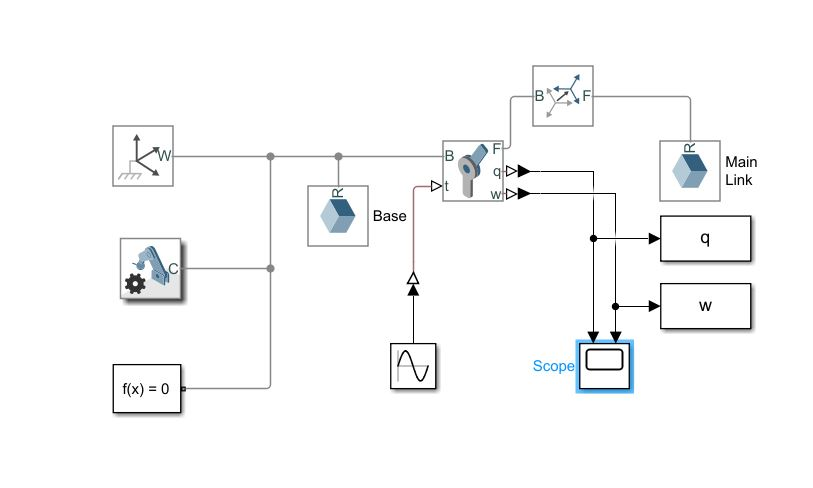
\includegraphics[width=0.7\linewidth]{model}
		\caption{Блок-схема модели}
		\label{fig:model}
	\end{figure}
	Основание -- куб, маятник -- параллелепипед:
	\begin{figure}[H]
		\centering
		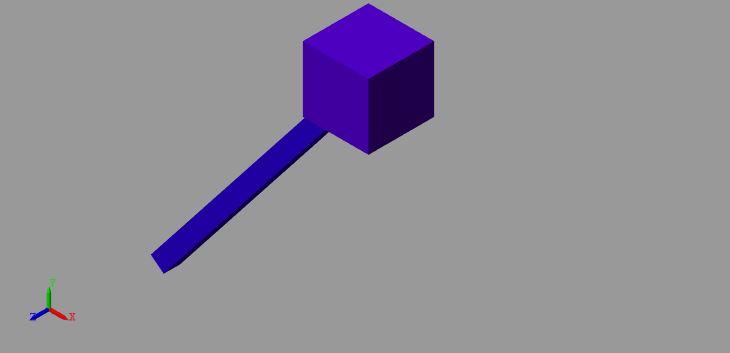
\includegraphics[width=0.7\linewidth]{pend1}
		\caption{Внешний вид маятника}
		\label{fig:pend1}
	\end{figure}
	\subsection*{Результаты моделирования}
	\paragraph{Моделирование свободных колебаний\\}
	Моделирование свободных колебаний без сопротивления:
	\begin{figure}[H]
		\centering
		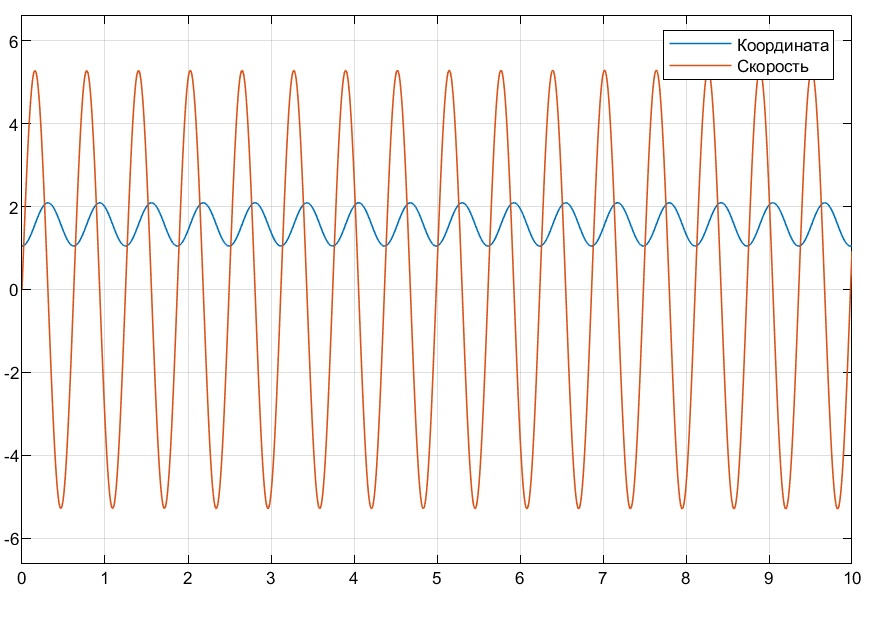
\includegraphics[width=0.7\linewidth]{coord1}
		\caption{График зависимости скорости и координаты от времени, $b = 0$, $\alpha = 60$}
		\label{fig:coord1}
	\end{figure}
	\begin{figure}[H]
		\centering
		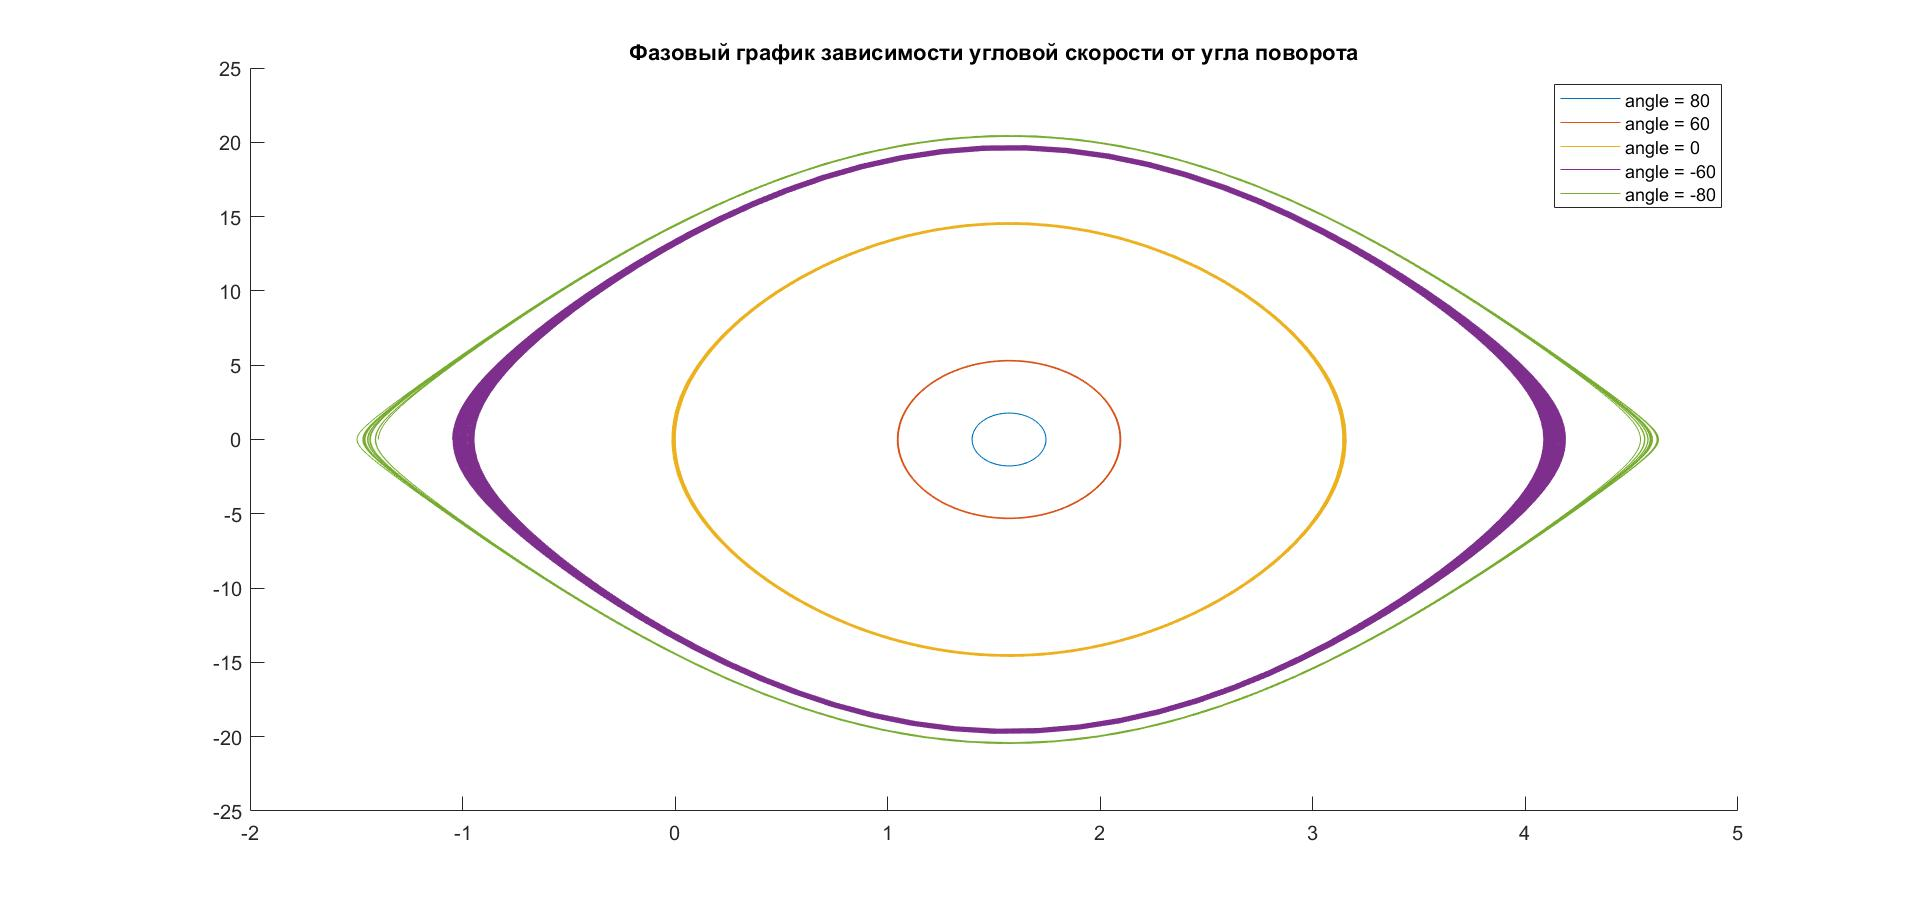
\includegraphics[width=1.2\linewidth]{phase1}
		\caption{Фазовый график зависимости угловой скорости от угла поворота для свободных колебаний без сопротивления при различных начальных углах отклонения [-80, -60, 0, 60, 80] и нулевой начальной скорости}
		\label{fig:phase1}
	\end{figure}
	Моделирование свободных колебаний с сопротивлением:
	\begin{figure}[H]
		\centering
		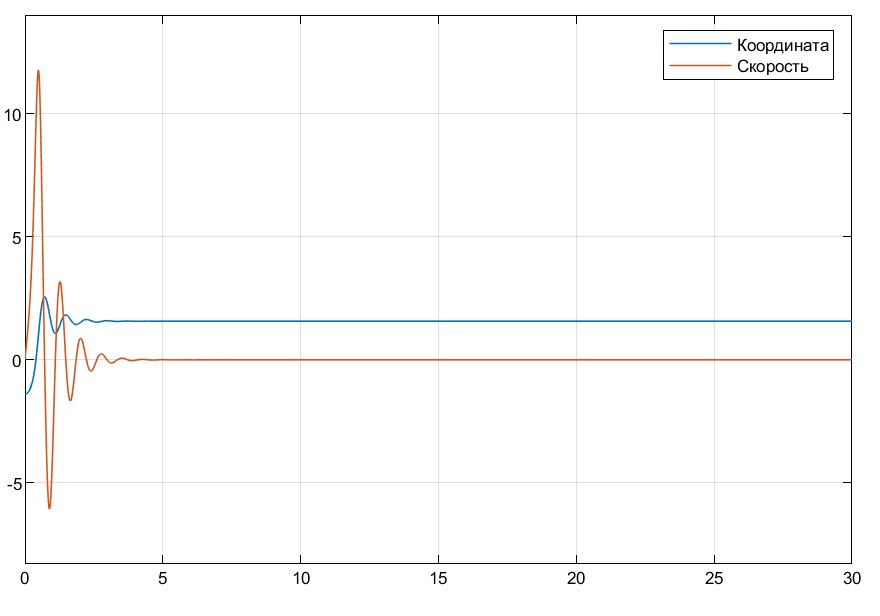
\includegraphics[width=0.7\linewidth]{coord2}
		\caption{График завиимости скорости и координаты от времени, $b = 8*10^{-5}$, $\alpha = 60$}
		\label{fig:coord2}
	\end{figure}
	\begin{figure}[H]
		\centering
		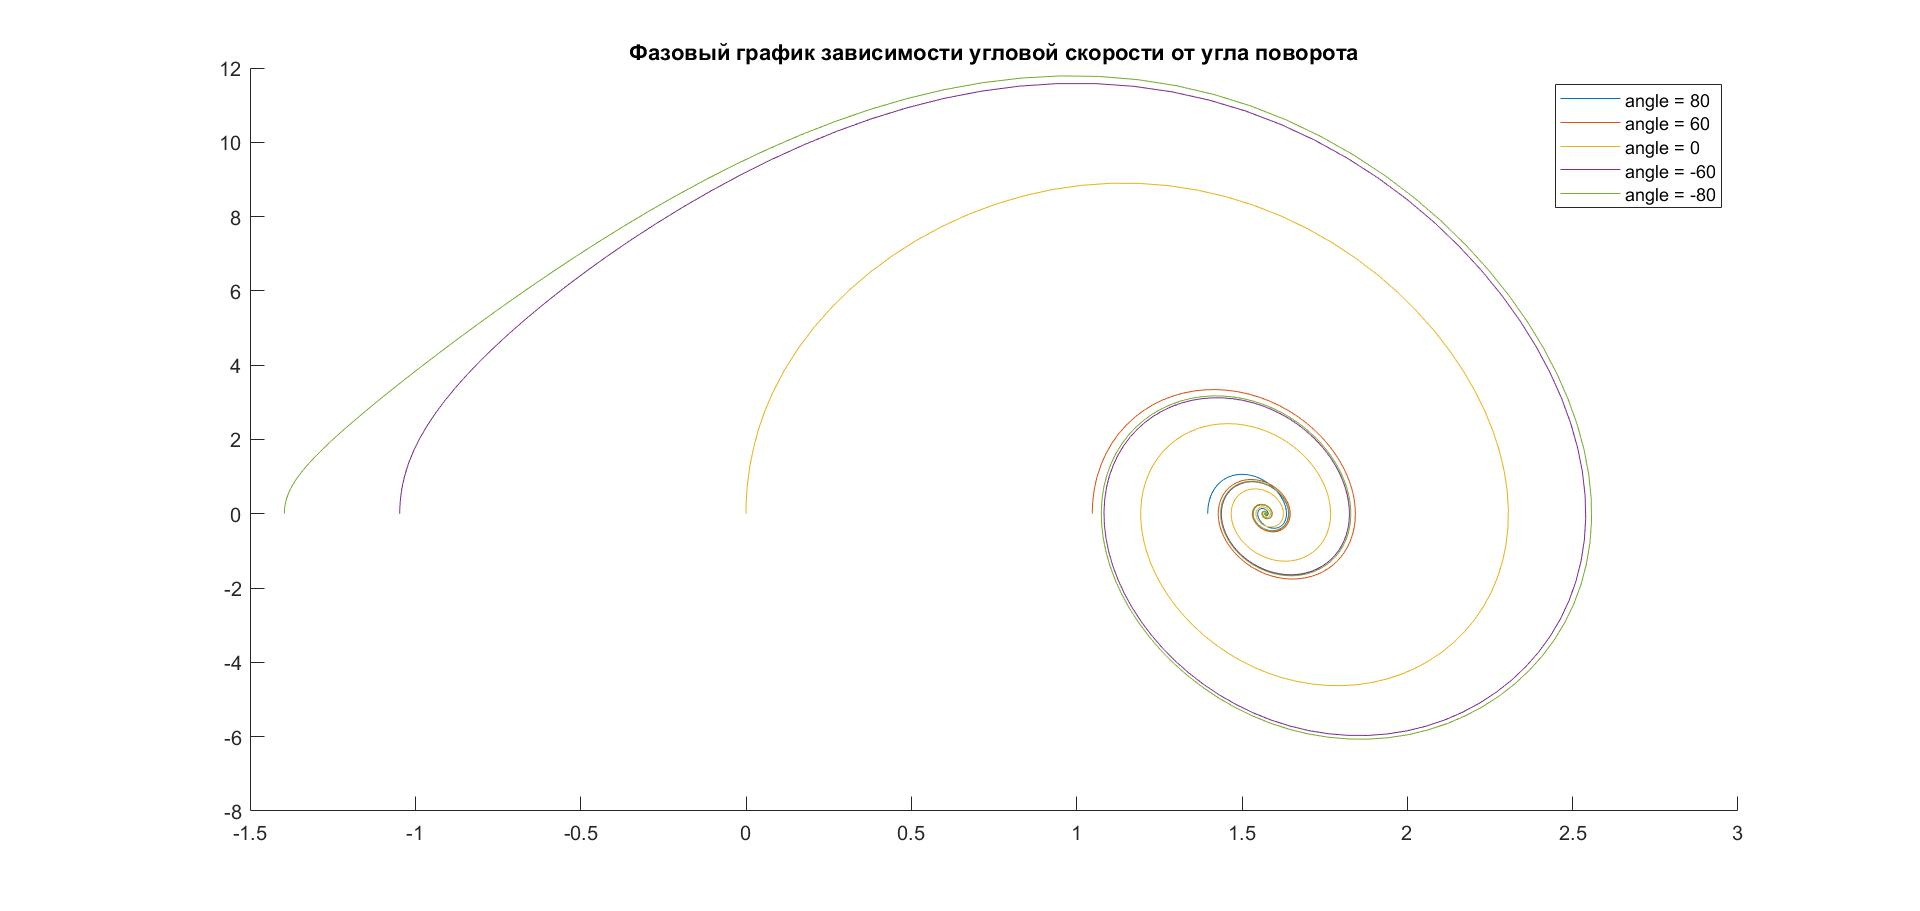
\includegraphics[width=1.2\linewidth]{phase2}
		\caption{Фазовый график зависимости угловой скорости от угла поворота для свободных колебаний c сопротивлением при различных начальных углах отклонения [-80, -60, 0, 60, 80] и нулевой начальной скорости}
		\label{fig:phase2}
	\end{figure}
	\paragraph*{Моделирование вынужденных колебаний\\}
	\begin{figure}[H]
		\centering
		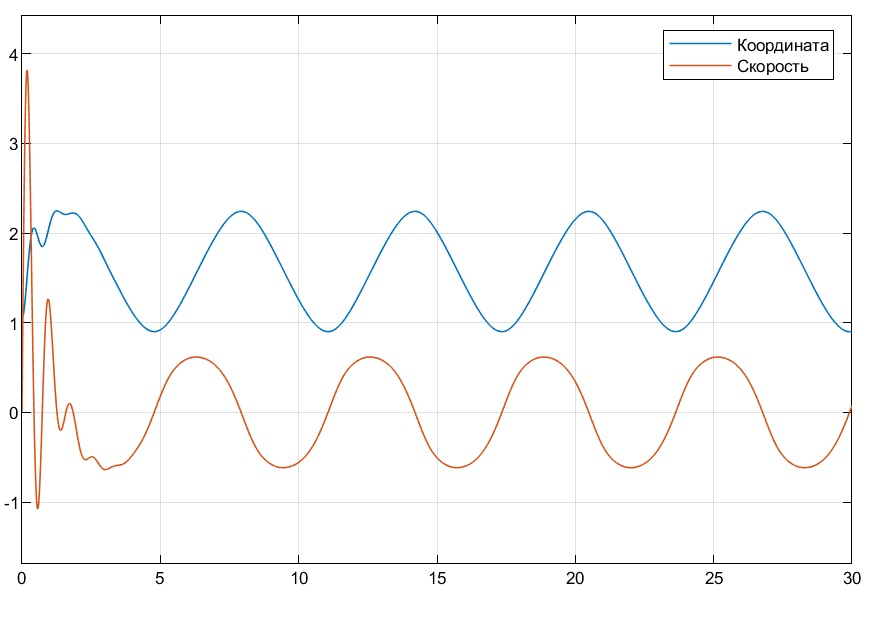
\includegraphics[width=0.7\linewidth]{coord3}
		\caption{Моделирование вынужденных колебаний, амплитуда $A = 0.06$, $\omega = 10$}
		\label{fig:coord3}
	\end{figure}
	\begin{figure}[H]
		\centering
		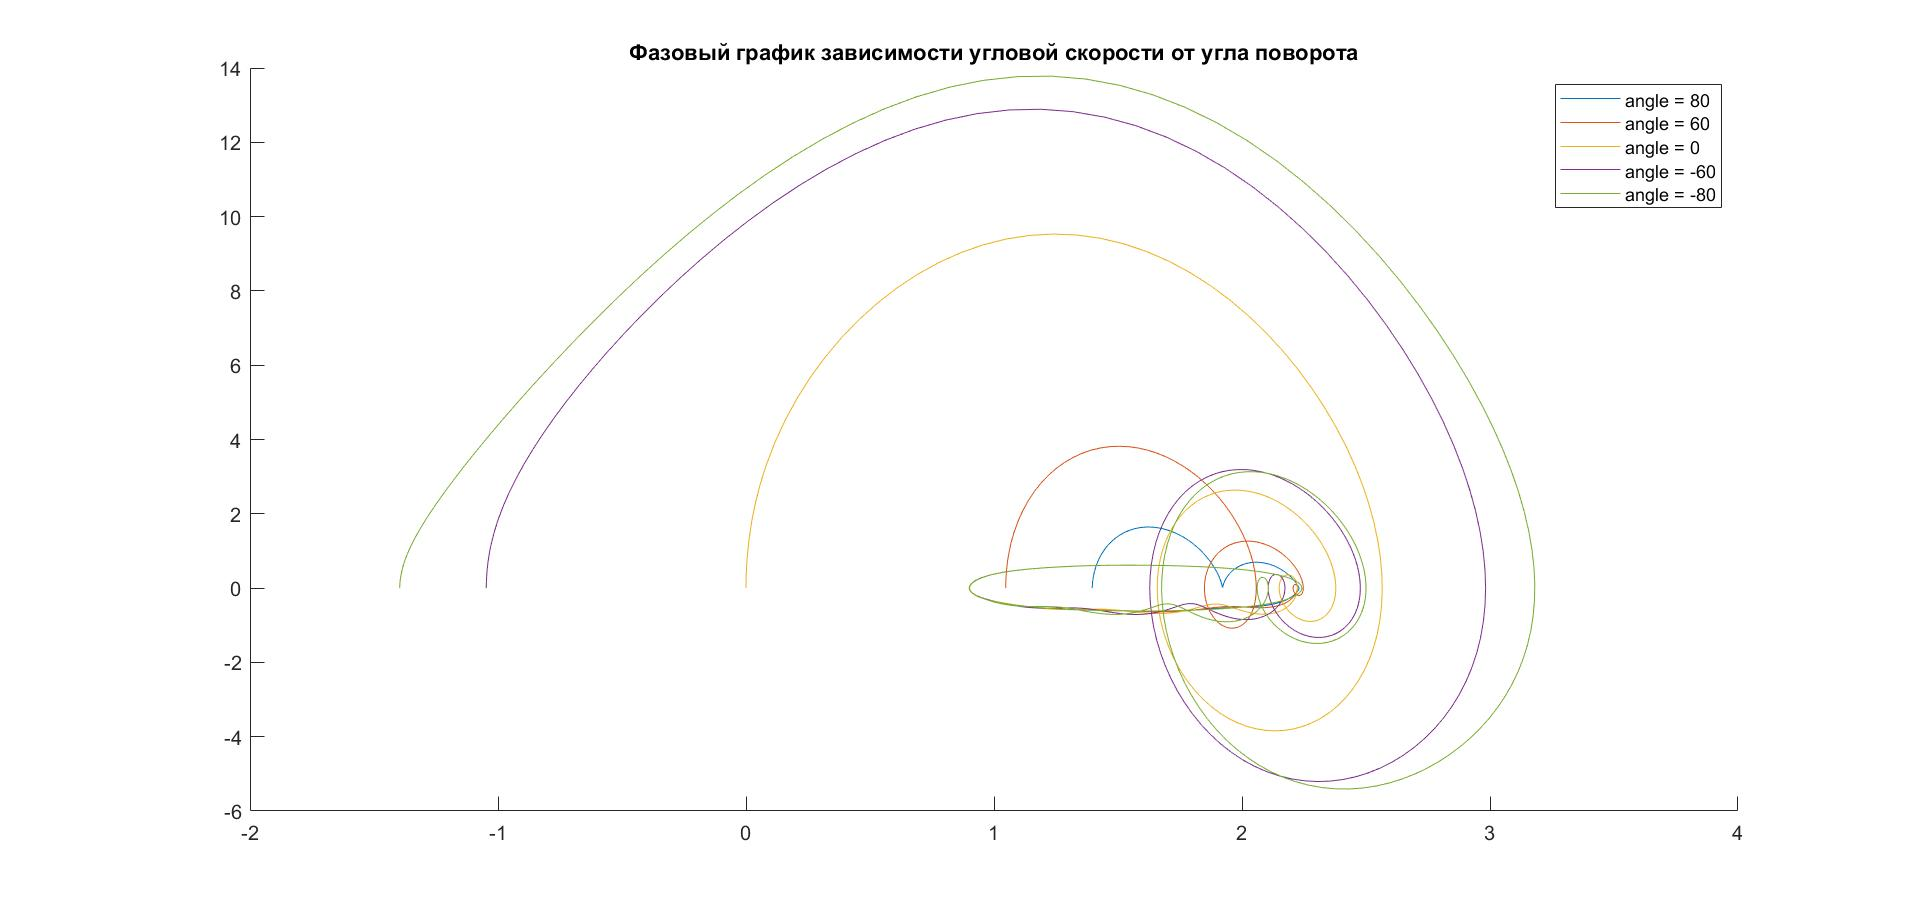
\includegraphics[width=1.2\linewidth]{phase3}
		\caption{Фазовый график зависимости угловой скорости от угла поворота для вынужденных колебаний c сопротивлением при различных начальных углах отклонения [-80, -60, 0, 60, 80] и нулевой начальной скорости, $A = 0.06$, $\omega = 10$}
		\label{fig:phase3}
	\end{figure}
	После этого в конструкцию маятника были внесены изменения -- изменена форма основания на девятигранник, форма звена изменена на эллипс. После внесения изменений было проведено моделирование вынужденных колебаний, значения плотности были оставлены такими же:
	\begin{figure}[H]
		\centering
		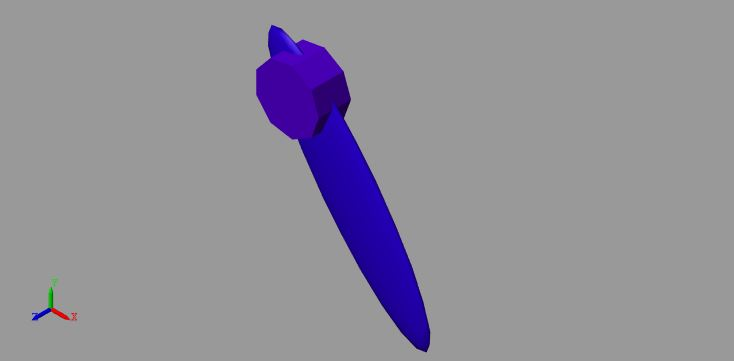
\includegraphics[width=0.7\linewidth]{pend2}
		\caption{Внешний вид измененного маятника}
		\label{fig:pend2}
	\end{figure}
	
	\begin{figure}[H]
		\centering
		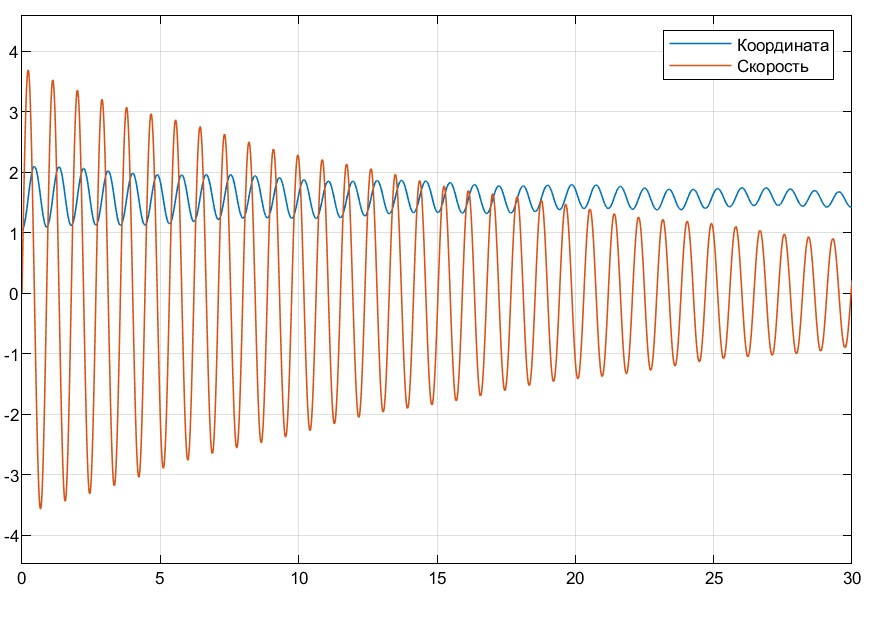
\includegraphics[width=0.7\linewidth]{coord4}
		\caption{Вынужденные колебания, параметры силы те же, $\alpha = 60$}
		\label{fig:coord4}
	\end{figure}
	\begin{figure}[H]
		\centering
		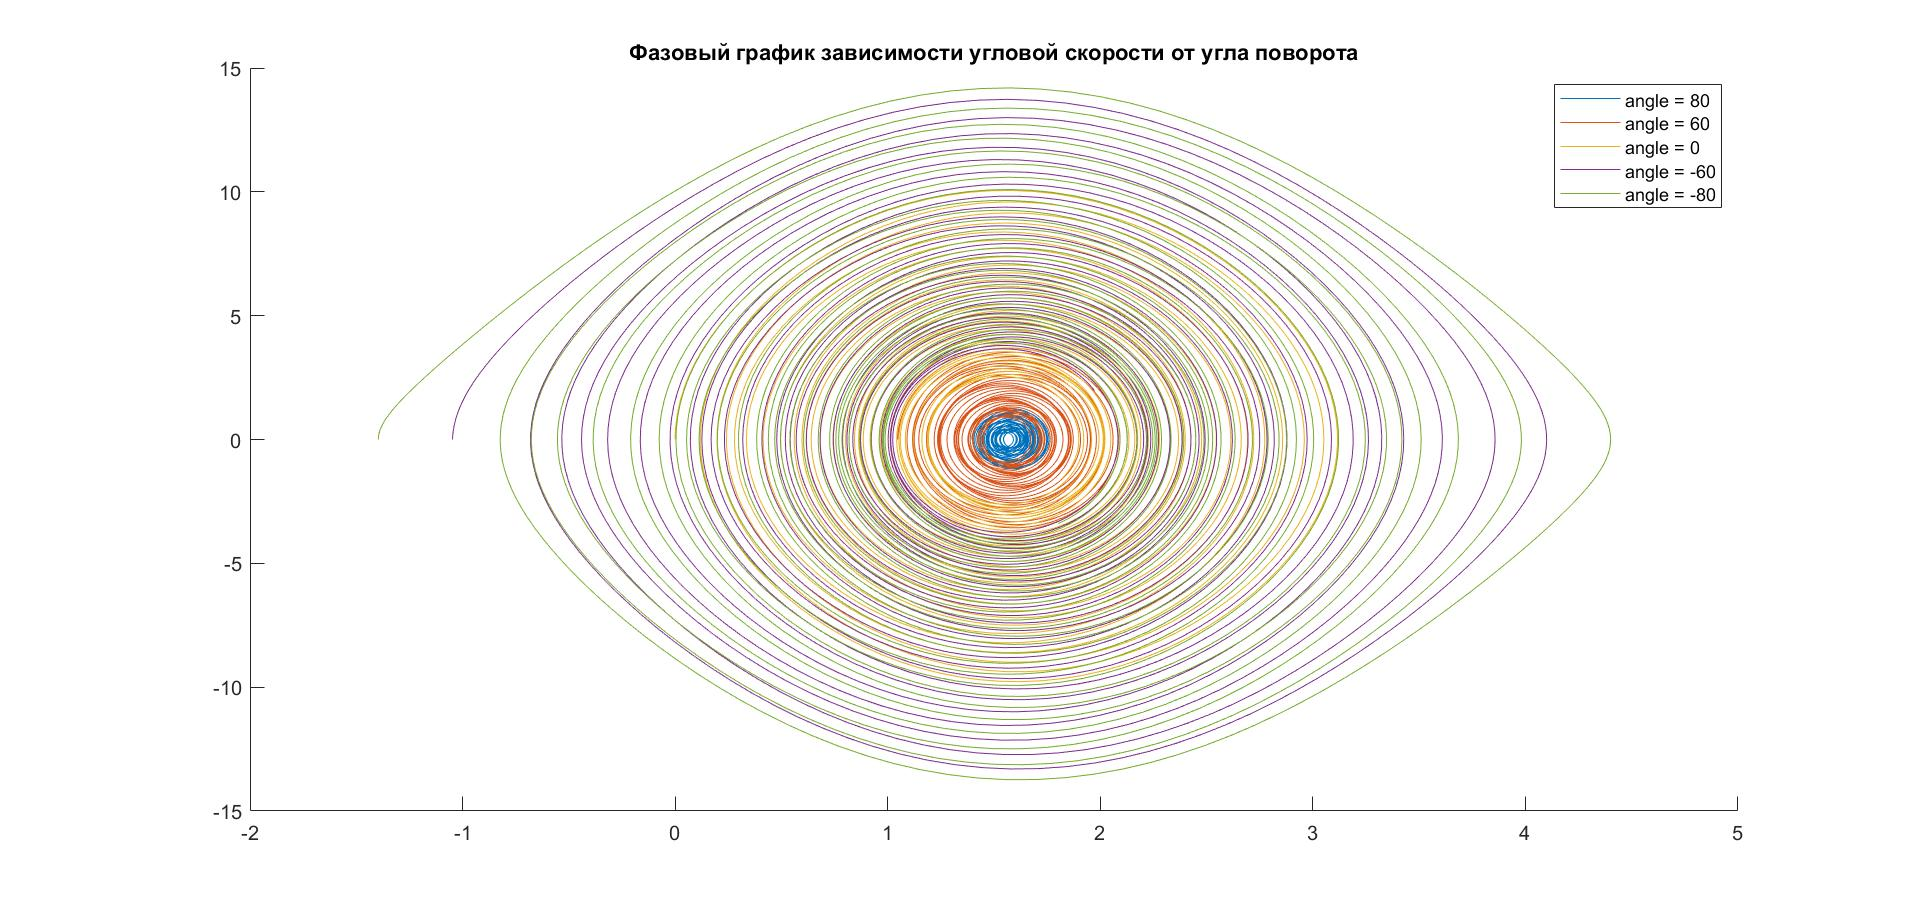
\includegraphics[width=1.2\linewidth]{phase4}
		\caption{Фазовый график зависимости угловой скорости от угла поворота измененного маятника для вынужденных колебаний c сопротивлением при различных начальных углах отклонения [-80, -60, 0, 60, 80] и нулевой начальной скорости, $A = 0.06$, $\omega = 10$}
		\label{fig:phase4}
	\end{figure}
	
\end{document}